


\usetikzlibrary{calc}



\newcommand{\drawgrid}[2]{%
\draw[line cap=rect] (0,0) grid ++ (#1,#2); 
}


\newcommand{\fillcoord}[2]{%

\fill[black] (#1,#2) rectangle ++ (1,1); 

}

\newcommand{\namecoord}[4]{%

\node[label=center:#4] (#3) at ($(#1,#2)+(0.5,0.5)$) {};

}


\newcommand{\selectcoord}[2]{%

\draw[color=red, line width=1pt, line cap=rect]  (#1,#2) grid ($(#1,#2)+(1,1)$) {}; 

}




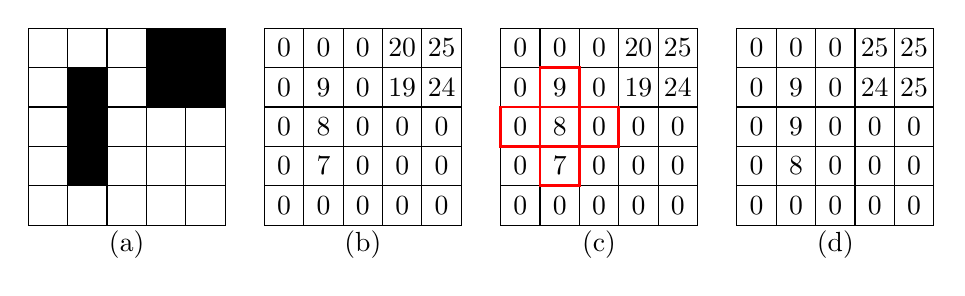
\begin{tikzpicture}[scale=0.5]







\drawgrid{5}{5}

\fillcoord{1}{1}
\fillcoord{1}{2}
\fillcoord{1}{3}


\fillcoord{3}{3}
\fillcoord{3}{4}
\fillcoord{4}{3}
\fillcoord{4}{4}


\namecoord{2}{-1}{}{(a)}


\drawgrid{5}{5}


\begin{scope}[shift={(6,0)}]
\namecoord{2}{-1}{}{(b)}

\foreach \i in {0,...,4}
\foreach \j in {0,...,4}
{
\namecoord{\i}{\j}{init\i\j}{0}
}

\node also [label={[fill=white]center:7}] (init11);
\node also [label={[fill=white]center:8}] (init12);
\node also [label={[fill=white]center:9}] (init13);


\node also [label={[fill=white]center:19}] (init33);
\node also [label={[fill=white]center:20}] (init34);
\node also [label={[fill=white]center:24}] (init43);
\node also [label={[fill=white]center:25}] (init44);



\drawgrid{5}{5}


\end{scope}

\begin{scope}[shift={(12,0)}]
\namecoord{2}{-1}{}{(c)}

\foreach \i in {0,...,4}
\foreach \j in {0,...,4}
{
\namecoord{\i}{\j}{init\i\j}{0}
}


\node also [label={[fill=white]center:7}] (init11);
\node also [label={[fill=white]center:8}] (init12);
\node also [label={[fill=white]center:9}] (init13);


\node also [label={[fill=white]center:19}] (init33);
\node also [label={[fill=white]center:20}] (init34);
\node also [label={[fill=white]center:24}] (init43);
\node also [label={[fill=white]center:25}] (init44);


\drawgrid{5}{5}



\selectcoord{0}{2}

\selectcoord{1}{1}
\selectcoord{1}{2}
\selectcoord{1}{3}

\selectcoord{2}{2}





\end{scope}

\begin{scope}[shift={(18,0)}]
\namecoord{2}{-1}{}{(d)}

\foreach \i in {0,...,4}
\foreach \j in {0,...,4}
{
\namecoord{\i}{\j}{init\i\j}{0}
}


\node also [label={[fill=white]center:8}] (init11);
\node also [label={[fill=white]center:9}] (init12);
\node also [label={[fill=white]center:9}] (init13);


\node also [label={[fill=white]center:24}] (init33);
\node also [label={[fill=white]center:25}] (init34);
\node also [label={[fill=white]center:25}] (init43);
\node also [label={[fill=white]center:25}] (init44);


\drawgrid{5}{5}

\end{scope}


\end{tikzpicture}



